\chapter{Агрегирование гетерогенных текстовых коллекций в тематической иерархии}
\section{Постановка задачи}

В данной работе решается задача агрегирования больших гетерогенных текстовых коллекций в их общей иерархической тематической модели.
Предполагается, что есть начальное приближение тематической иерархии, в котором уже присутствует большинство агрегируемых тем. 

Назовем коллекцию, модель которой берется за начальное приближение, базовой. Такая модель должна быть хорошо интерпретируемой.
Алгоритм, решающий поставленную задачу, должен позволить увеличивать объем и разнообразие агрегируемого контента, добавляя в модель базовой коллекции документы из других источников. При этом конечный размер агрегируемой коллекции может во много раз превышать размер базовой коллекции. Кроме того, модель должна оставаться интерпретируемой и как можно меньше терять в качестве по сравнению с моделью базовой коллекции. 

Вычислительный эксперимент в данной работе должен проводиться на текстовых коллекциях из нескольких источников, которые существенно отличаются друг от друга по размеру и набору тем. Такие коллекции позволяют исследовать работу предлагаемого метода на гетерогенных данных.

В качестве примера в этой работе рассматривается задача агрегирования русскоязычного научно-популярного контента из коллекций, описанных в секции 3.2.1.
 Будем использовать коллекцию ПостНауки в качестве базовой, так как она содержит разнородные темы (технические, естественнонаучные и гуманитарные), поэтому для большинства научно-популярных статей в ней найдутся тематически близкие документы. При этом она сравнительно мала по объему.
Коллекция Хабрахабра напротив содержит в основном технические статьи, меньше естественнонаучных и почти не содержит гуманитарных. При этом ее объем во много раз превышает объем коллекции ПостНауки, взятой за базовую. Таким образом, на примере этих коллекций можно оценить эффективность алгоритмов для задачи агрегации.

\section{Базовый алгоритм}

Стандартный алгоритм построения тематической модели гетерогенных текстовых коллекций предполагает объединение коллекций из разных источников и построение общей модели. В этом эксперименте объединяются коллекции ПостНауки и Хабрахабра.

В силу того, что размер коллекции Хабрахабра существенно превосходит размер коллекции ПостНауки, в большинстве тем полученной модели более 90\% статей относятся к Хабрахабру.

\begin{table}[h!]
\centering
\vspace{1ex}
\begin{tabular}{l|r|r|r|r|r|r|r|r|r|r|r}

$t$ & 0 & 1 & 2 & 3 & 4 &5 & 6 & 7 & 8 & 9 & 10\\
\hline
$P_t$ & 0.94 &  0.79 & 0.97 & 0.98 & 0.91 & 0.95 & 0.98& 0.99 & 0.92 &  0.95 &  0.98 \\
\hline
\hline
$t$ & 10 & 11 & 12  &13 & 14 & 15 & 16 & 17  &18 & 19 & 20\\
\hline
$P_t$ & 0.98 &  0.91 & 0.99 &  0.93 &  0.98  & 1.0 & 0.97 &  0.97  &0.99 & 0.97 & 0.95\\
\end{tabular}
\caption{\label{table:baseline}Доля статей Хабрахабра в темах модели объединенной коллекции. $t$ -- номер темы, $P_t$ -- доля статей Хабрахабра в этой теме, если к теме относятся документы с $p(t|d) > 0.1$.}
\end{table}

Поэтому модель объединенной коллекции отражает в основном тематическую структуру Хабрахабра. Все темы имеют технический характер, характерный для него. При этом потеряны гуманитарные темы, представленные в ПостНауке.
Кроме того, объединенная коллекция имеет большой размер, поэтому для построения ее модели требуется намного больше времени, чем для построения модели ПостНауки.
Таким образом, базовый алгоритм не решает поставленную задачу и требует модификаций.

\section{Предлагаемый алгоритм}

В данной работе для решения поставленной задачи предлагается проводить построение модели в несколько этапов. Обозначим базовую коллекцию как $D_0$, а коллекцию, состоящую из документов, которые необходимо добавить к агрегируемому контенту, как $D_1$. Тогда предлагаемый метод можно описать следующим образом:

\begin{enumerate}
	\item \textbf{Начальное приближение}: построить модель базовой коллекции $D_0$. Параметры модели начального приближения обозначим как $\Phi_0^l$, $\Theta_0^l$, где $l$ -- номер уровня. 
	\item \textbf{Фильтрация}: отранжировать документы добавляемой коллекции $D_1$ в порядке уменьшения близости к базовой коллекции $D_0$ в смысле некоторой метрики.
	
	\item \textbf{Дополнение модели:} добавить выбранное количество документов $D_1$, отранжированных в начало списка на этапе фильтрации, в коллекцию. При этом получим новую коллекцию $D$. Инициализировать параметры $\Phi^l$ модели коллекции $D$ параметрами $\Phi_0^l$ начального приближения. Обучить иерархическую модель $D$.
	 
\end{enumerate}

Первый этап -- задача построения интерпретируемой тематической иерархии однородной коллекции. Эта задача рассмотрена в \cite{hARTM}, кроме того, в \cite{Ianina2017} рассмотрена задача подбора коэффициентов регуляризации в модели ARTM. 

Опишем подробнее два последних этапа.

\subsection{Фильтрация новой коллекции}
Целью этого этапа является сокращение объема добавляемой коллекции (отфильтрованная коллекция должна содержать меньше документов, чем уже содержится в построенной модели) и удаление статей, которые далеки по содержанию от уже присутсвующих в модели. Это позволяет отобрать статьи, которые необходимо агрегировать и отсеять те, которые являются нерелевантными.

Фильтрацию предлагается проводить по расстоянию новых документов до ближайших документов из старой коллекции. Это расстояние можно рассчитывать по разным метрикам близости документов. В этой работе будем использовать косинусное расстояние между их tf-idf-представлениями, где idf берется по старой коллекции.

Пусть $\boldsymbol{d_n }= [ \text{tf}(w_i, d_n) \cdot \text{idf}(w_i, D_0) ]_{i=1}^{|W|}$, где $D_0$ --- базовая коллекция, $D_1$ --- добавляемая коллекция, $w_i \in W$ --- токены из словаря базовой коллекции $W$, $d_n \in D_0 \cup D_1$ --- документ.

Расстояние между документами $d_n$ и $d_m$ рассчитывается как их косинусное сходство:
$$\rho(d_n, d_m) = \dfrac{\boldsymbol{d_n }^T \boldsymbol{d_m }}{||\boldsymbol{d_n }|| \cdot ||\boldsymbol{d_m }||}.$$

Для каждого документа $d_n \in D_1$ можно найти 10 ближайших документов из коллекции $D_0$. Пусть этим документам соответствуют индексы $[m_1, ..., m_{10}]$. Тогда искомая отфильтрованная выборка состоит из тех документов $d_n$, для которых выполняется условие

$$\tfrac{1}{10}\sum_{m \in [m_1, ..., m_{10}]}\rho(d_n, d_m) < t,$$
где $t$ -- некоторое заданное пороговое сходство между документами.

Обозначим отфильтрованную коллекцию, состоящую из документов, удовлетворяющих данному условию, как $D_f$.

\subsection{Дополнение модели отфильтрованной коллекцией}
На этом этапе полученная выборка документов добавляется в модель начального приближения иерархии. 
При этом предполагается, что начальное приближение уже содержит все темы, характерные для агрегируемого контента. Тогда процесс добавления новых документов можно описать следующим образом:

\begin{enumerate}
	\item \textbf{Слияние коллекций:} добавить отфильтрованную коллекцию к базовой и получить объединенную коллекцию $D = D_0 \cup D_f$.
	\item \textbf{Инициализация:} после добавления новых документов строки новых матриц $\Phi^l$ иерархии коллекции $D$, соответсвующие токенам старого словаря, не должны значительно отличаться от соответствующих строк старой матрицы $\Phi^l_0$. Будем строить модель, используя только словарь базовой коллекции. Поэтому инициализируем матрицы $\Phi^l$ соответствующими матрицами $\Phi^l_0$.  
	\item \textbf{Обучение иерархии:} используем модель hARTM для построения иерархической тематической модели коллекции $D$. На каждом уровне иерархии начальные значения параметров заданы на этапе инициализации.
\end{enumerate}


\section{Вычислительный эксперимент: агрегирование русскоязычного научно-популярного контента}
\todo{построить визуализации}
Опишем реализацию предложенного метода для задачи агрегирования русскоязычного научно-популярного контента на примере коллекций ПостНауки и Хабрахабра.

\subsection{Начальное приближение: иерархия ПостНауки} 

Первый этап --- построение модели ПостНауки, в которую в дальнейшем планируется добавлять документы Хабрахабра. 

 Модель содержит два уровня иерархии. На первом уровне 21 тема (одна фоновая). На втором уровне 61 тема (1 фоновая). Использовались модальности слов и тэгов, причем для тэгов был установлен значительно больший вес, что позволило существенно улучшить качество модели.

\textbf{Первый уровень иерархии}

Применялись регуляризаторы декорреляции терминов нефоновыx тем и сглаживания $\Phi$ для фоновой темы.

\begin{figure}[h]
    \centering 
    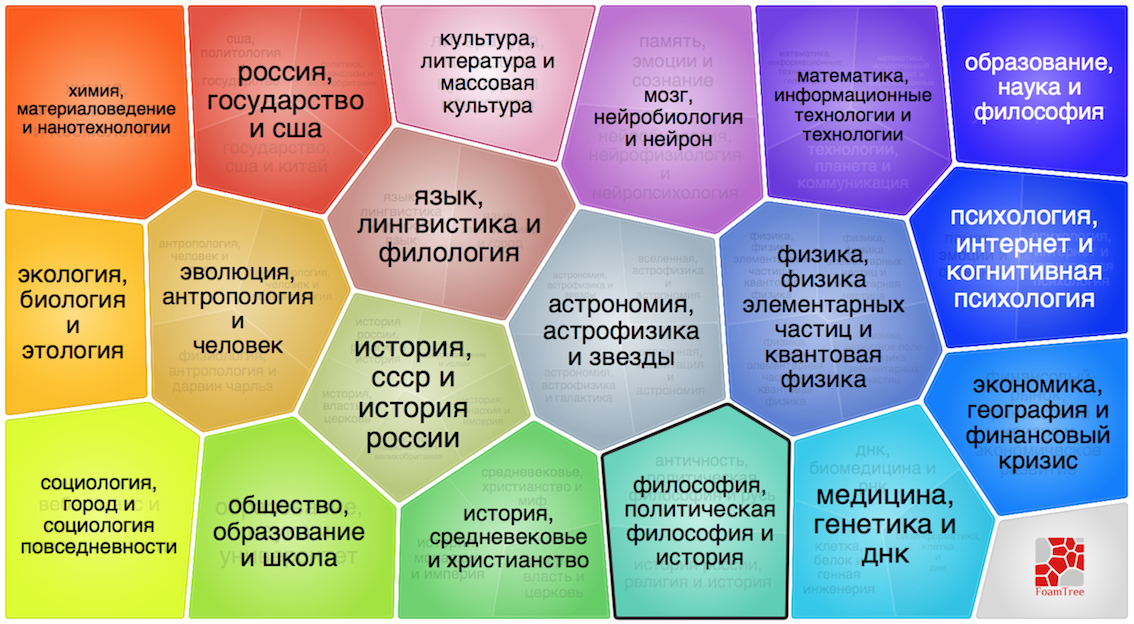
\includegraphics[width=1\textwidth]{img/pn_level0.png}
    \caption{\label{fig:pn_level0}Визуализация первого уровня иерархии ПостНауки}
\end{figure}

На рисунке \ref{fig:pn_level0} изображена визуализация полученной модели. В названия тем вынесены 3 наиболее вероятных для данной темы токена. 


\textbf{Второй уровень иерархии}
 
\begin{figure}[h]
    \centering 
    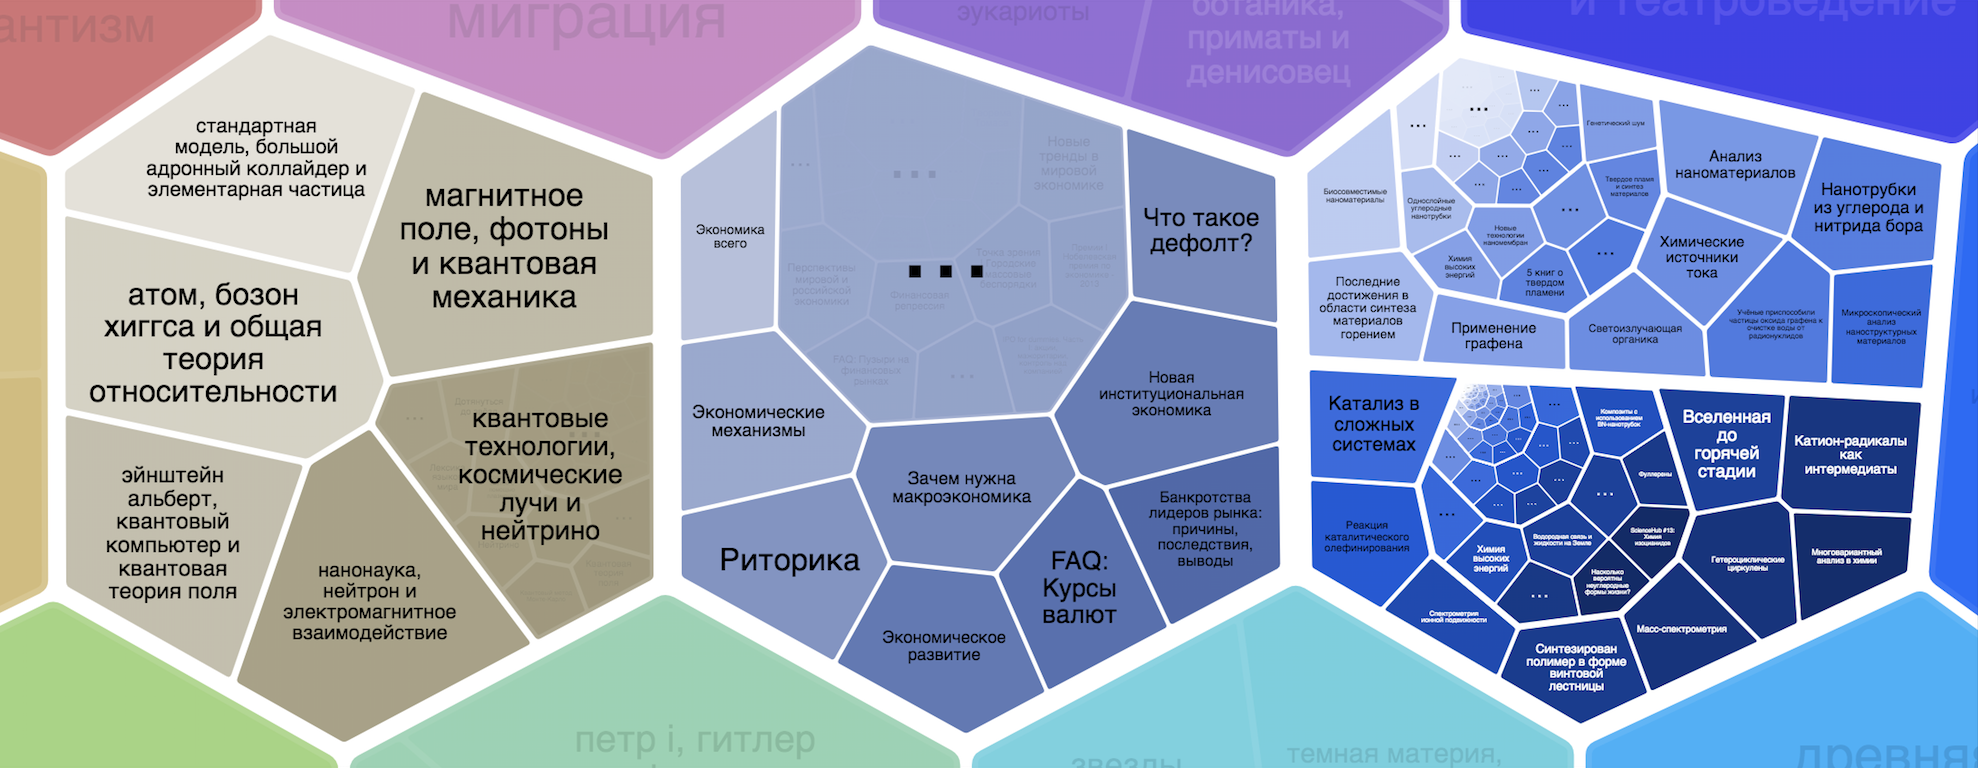
\includegraphics[width=1\textwidth]{img/pn_level1.png}
    \caption{\label{fig:pn_level1}Визуализация уровней иерархии ПостНауки. Первый и второй уровень содержат темы, на третьем уровне находятся отнесенные к темам документы.}
    \end{figure}

Применялась следующая стратегия регуляризации: 
\begin{itemize} \item первые 10 итераций применялись регуляризаторы декорреляции терминов нефоновых тем и сглаживания $\Phi$ фоновой темы;

\item после 10 итераций подмножества нефоновых тем, которые модель отнесла к одной родительской теме первого уровня, разреживались с помощью регуляризатора разреживания $\Theta$ между собой с коэффициентами $\tau$, возрастающими с каждой итерацией и пропорциональными количеству тем в каждом подмножестве.
\end{itemize}

На рисунке \ref{fig:pn_level1} изображены различные уровни иерархии в полученной модели, темы проименованные тремя наиболее вероятными токенами.

Полученная модель содержит существенно различные темы в силу того, что контент ПостНауки разнородный (содержит как естественнонаучные, так и гуманитарные и технические статьи). В дальнейшем будем предполагать, что в ней содержатся все характерные для научно-популярных статей темы. 

\subsection{Фильтрация коллекции Хабрахабра} 
Коллекция Хабрахабра была отранжирована по предложенной метрике близости. Затем полученные значения расстояний были отнормированы по метрике max. Было выбрано значение порогового расстояния $t = 0.85$. При этом в отфильтрованную коллекцию $D_f$ вошло 9288 документов, то есть размер добавленной коллекции в несколько раз превышает размер базовой коллекции. 


\subsection{Дополнение модели ПостНауки отфильтрованной коллекцией Хабрахабра}
Модель содержит два уровня иерархии. На первом уровне 21 тема (одна фоновая). На втором уровне 61 тема (1 фоновая).
Объединенная коллекция $D = D_0 \cup D_f$ содержит 12264 документа. 

\textbf{Первый уровень иерархии} 

$\Phi^1$ инициализировалась, как описано в алгоритме.
Применялись регуляризаторы декорреляции терминов нефоновыx тем с коэффициентом, увеличенным пропорционально увеличению размера коллекции и сглаживания $\Phi$ для фоновой темы.

На рис.4 изображена визуализация полученной модели. Видно, что полученная модель отличается от первого уровня иерархии
ПостНауки незначительно. Таким образом, добавленные документы из коллекции Хабрахабра распределились по существующим темам.

\begin{figure}[h]
    \centering 
    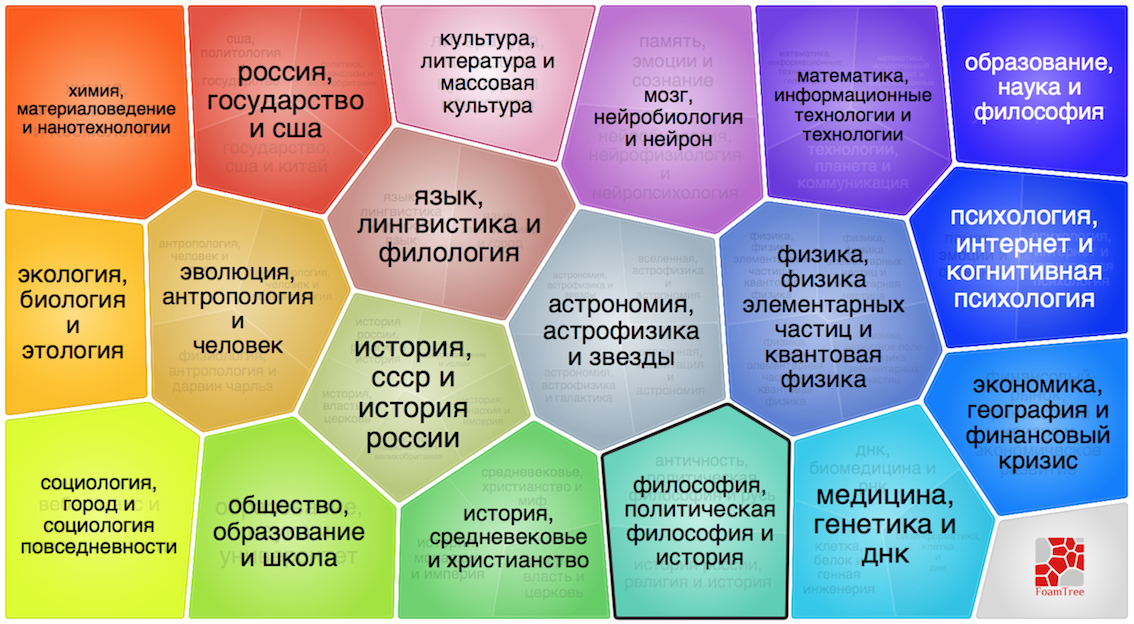
\includegraphics[width=1\textwidth]{img/pn_level0.png} \\
 \caption{Визуализация первого уровня иерархии}
    \end{figure}
    
\begin{table}[h]
\centering
\begin{tabular}[t]{p{22em}|p{2em}|p{2em}}
 Название темы $t$ & $|D_t|$ & $P_t$\\
\hline
\textit{'технологии', 'интернет', 'социальные сети'} & 6006& 0.95 \\
\hline
\textit{'математика', 'статистика', 'нейронные сети'} & 2434 & 0.93 \\
\hline
\textit{'экономика', 'сша', 'япония'} & 2203& 0.90  \\
\hline
\textit{'право', 'юриспруденция', 'закон'} & 1463&  0.92  \\
\hline
\textit{'образование', 'наука', 'университет'} & 1298& 0.86  \\
\hline
\textit{'философия', 'история философии', 'политическая философия'} & 142& 0.34  \\
\hline
\textit{'медицина', 'биомедицина', 'онкология'} &120& 0.28 \\
\hline
\textit{'биология', 'эволюция', 'днк'} & 111 & 0.15  \\
\hline
\textit{'история', 'история россии', 'средневековье'} & 94& 0.15  \\

\end{tabular}
\caption{\label{table:p_habr}Распределение новых документов по темам. $|D_t|$ -- количество документов Хабрахабра, отнесенных к теме $t$ по порогу вероятности $p(t|d) > 0.1$. $P_t$ -- доля документов Хабрахабра среди всех документов темы $t$}
\end{table}

\textbf{Второй уровень иерархии} 

$\Phi^2$ инициализировалась, как описано в алгоритме.

На втором уровне иерархии использовалась та же стратегия регуляризации, что и для второго уровня модели базовой коллекции. Коэффициент при декоррелирующем регуляризаторе был также изменен пропорционально размеру коллекции. 

В таблице \ref{table:p_habr} приведены темы построенной модели с соответствующими им количеством и долей статей Хабрахабра. Таблица содержит все темы с наибольшим количеством статей Хабрахабра и несколько примеров тем с малой долей статей Хабрахабра. Как и ожидалось, добавленные документы распределились по темам, характерным для Хабрахабра. При этом темы, характерные только для ПостНауки, содержат значительно меньше статей Хабрахабра. Так как объединенная коллекция содержит в основном документы Хабрахабра, такое распределение приводит к существенным различиям в размере тем, тогда как при базовом подходе к построению модели все темы имеют примерно одинаковый размер.

\section{Сравнение алгоритмов}

Предлагаемый метод построения тематической иерархии имеет несколько существенных отличий от базового метода: выбор множества добавляемых документов с помощью фильтрации, использование словаря базовой коллекции, инициализация начальных значений параметров модели. Для исследования того, как эти отличия влияют на качество иерархии, приведем сравнительный анализ нескольких модификаций предлагаемого алгоритма и базового алгоритма. Будем оценивать качество каждого алгоритма по метрикам качества иерархий, предложенным в секции 3.4.

Будем сравнивать модификации алгоритмов на одном и том же размере объединенной коллекции $D$, то есть в каждом случае в базовую коллекцию добавляется одинаковое количество документов $D_1$. Каждая рассматриваемая модификация алгоритма может использовать или не использовать фильтрацию (\textbf{Ф}), сокращение словаря до словаря базовой коллекции (\textbf{С}) и инициализацию параметров (\textbf{И}). Тогда опишем в таком виде исследуемые модификации.

\begin{itemize}
	\item \textbf{Ф- С- И-}. Это базовый алгоритм. В качестве $D_f$ выбирается случайное подмножество статей $D_1$ и строится модель объединенной коллекции $D = D_0 \cup D_f$. 
	\item \textbf{Ф+ С- И-}. Для получения $D_f$ используется фильтрация, описанная в секции 4.3.1, далее строится модель объединенной коллекции $D = D_0 \cup D_f$. 
	\item \textbf{Ф- С+ И-}. Предварительно находится словарь базовой коллекции. В качестве $D_f$ выбирается случайное подмножество статей $D_1$.  Модель строится только по словам из словаря $D_0$.
	\item \textbf{Ф- С- И+}. Предварительно строится модель базовой коллекции. В качестве $D_f$ выбирается случайное подмножество статей $D_1$. Модель объединенной коллекции $D = D_0 \cup D_f$ строится с инициализацией параметрами начального приближения.
	\item \textbf{Ф- С+ И-}. Предварительно находится словарь базовой коллекции. Для получения $D_f$ используется фильтрация, описанная в секции 4.3.1. Модель строится только по словам из словаря $D_0$.
	\item \textbf{Ф+ С+ И+-}. Это итеративная модификация предлагаемого алгоритма, в которой новые документы добавляются в коллекцию малыми порциями итеративно . При этом на каждой итерации за начальное приближение берется модель с предыдущей итерации. Таким образом, на каждой итерации матрица для инициализации параметров отличается от предыдущей.
	\item \textbf{Ф- С+ И+}. В качестве $D_f$ выбирается случайное подмножество статей $D_1$. Для инициализации используется модель базовой коллекции, модель строится только по словам словаря $D_0$.
	\item \textbf{Ф+ С+ И+}. Это предлагаемый алгоритм.

\end{itemize}

\begin{figure}[h]
    \centering 
    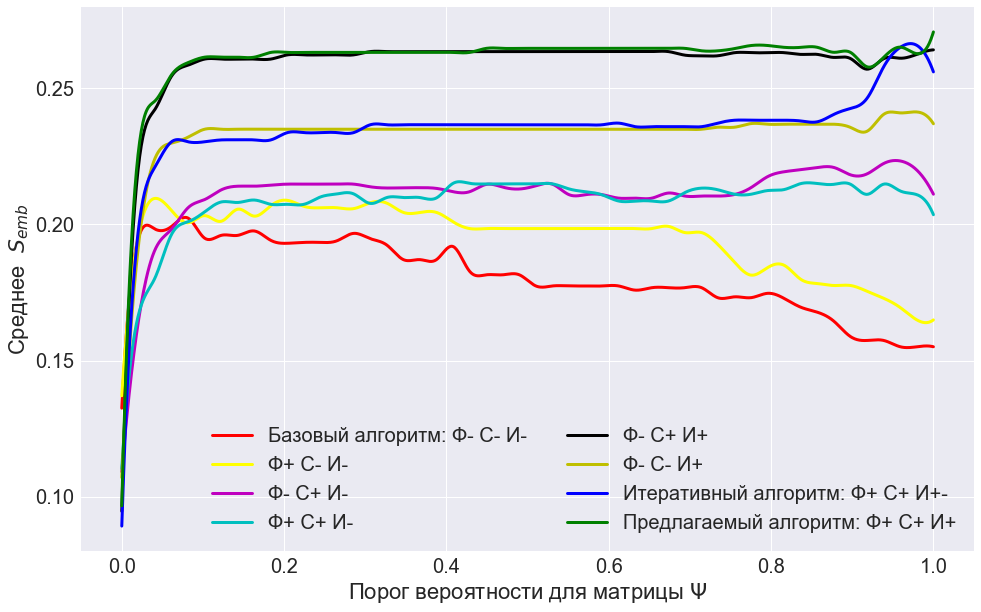
\includegraphics[width=1\textwidth]{img/alg_comparison.png}
    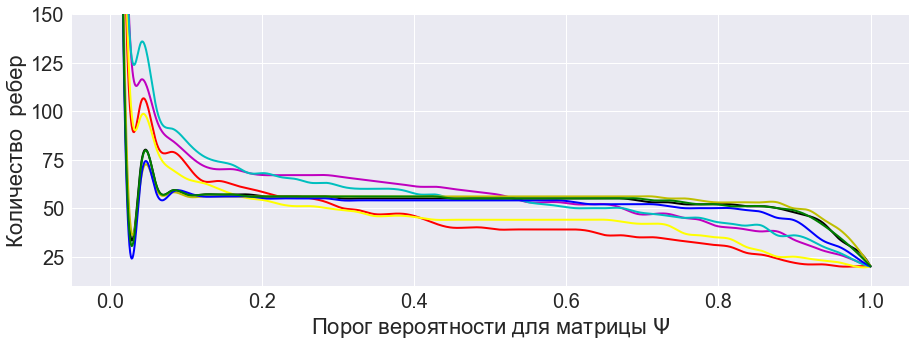
\includegraphics[width=1\textwidth]{img/num_edges.png}
    \caption{\label{fig:alg_comparison}Сравнение среднего качества ребер иерархии по метрике $\mathrm{S}_{emb}$ для исследуемых алгоритмов.}
\end{figure}

На графике \ref{fig:alg_comparison} приведено сравнение среднего значения метрики $\mathrm{S}_{emb}$ для каждого из описанных алгоритмов, как предложено в секции 3.4.1. На графике \ref{fig:rank_comparison} эти же алгоритмы сравниваются с помощью метрик качества ранжирования, описанных в секции 3.4.2, с использованием метрики $\mathrm{S}_{emb}$. Во всех алгоритмах гиперпараметры моделей и размер добавляемой коллекции были такими же, как в вычислительном эксперименте, описанном в секции 4.4. В итеративном алгоритме на каждой итерации в коллекцию добавлялось количество документов равное 10\% от размера коллекции на предыдущей итерации. Таким образом для добавления всей выборки $D_f$ понадобилось 19 итераций.

\begin{figure}
    \centering 
    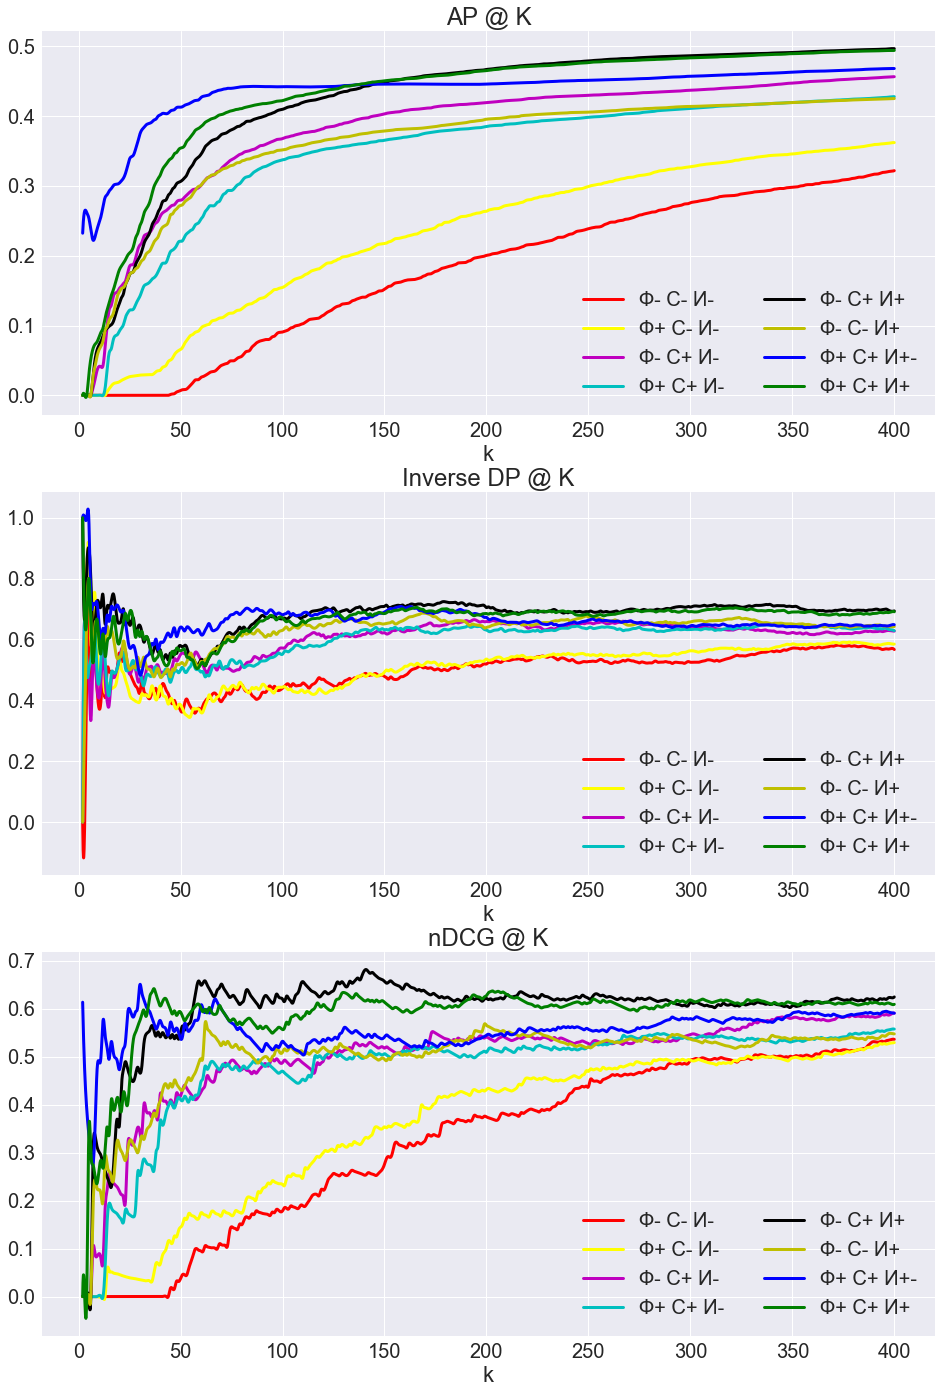
\includegraphics[width=1\textwidth]{img/ranking_alg_comparison.png}
    \caption{\label{fig:rank_comparison} Сравнение алгоритмов по метрикам качества ранжирования. Верное ранжирование задает метрика $\mathrm{S}_{emb}$.}
\end{figure}

На графике \ref{fig:alg_comparison} стоит рассматривать области низких и высоких порогов вероятности отдельно. В области высоких порогов усреднение метрики идет только по нескольким самым вероятным ребрам в иерархии, то есть по тем, которые модель считает наилучшими. В области низких порогов усреднение идет по большому количеству ребер. Для наглядности на графике \ref{fig:alg_comparison} снизу изображены зависимости количества ребер в иерархиях от порога. Видно, что для алгоритмов с лучшим качеством количество ребер изменяется слабо в широкой области порогов вероятности. Это можно считать показателем качества иерархии, так как в таком случае иерархия разрежена и почти все ненулевые значения значительно больше нуля. Если среднее качество падает с увеличением порога, как для базового алгоритма, это говорит о том, что алгоритм плохо ранжирует ребра иерархии. Это подтверждается метриками качестве ранжирования на графике \ref{fig:rank_comparison}.

Из приведенных результатов видно, что все три модификации базового алгоритма (фильтрация, словарь и инициализация) по отдельности улучшают качество иерархии. При этом наибольший прирост качества дает хорошая инициализация модели, меньший прирост дает сокращение словаря и меньше всего влияет на качество модели фильтрация. Видно, что фильтрация по tf-idf близости существенно не меняет модель, которая уже использует отфильтрованный словарь. Однако, используемые метрики качества говорят только о качестве тем и связей между темами. В случае модели без фильтрации в выборку попадают документы, которые плохо тематизируются и не относятся ни к одной из нефоновых тем со значимой вероятностью. Хотя это может не влиять значительно на качество модели по используемым метрикам, это нежелательный эффект, с которым помогает справится фильтрация.  

Наилучшее качество показывает предлагаемый алгоритм, почти такое же качество модели получается без фильтрации. Если использовать алгоритм итеративно с изменением параметров инициализации, то качество ухудшается, то есть лучшей стратегией является инициализация начальным приближением даже в случае, когда данные приходят порциями и алгоритм необходимо применять много раз.


